\documentclass[../main.tex]{subfiles}

\begin{document}

\section{Modello solare.}

\subsection{Per punti}

\tool{

\begin{itemize}
\item SSM: Description of solar interior reproducing observed properties with obs. error (Phis/chim input within uncertainties).
\item Before helioseismology: initial abundances $Y_0, Z_0,\alpha\xrightarrow{SSM}\rsun{},\lsun{},Z_{\odot}^{ph}$.
\item Simmetria sferica. Inclusione rotazione nella struttura idrostatica?
\item Stellar evolution : solar model - Observed properties
\item \sout{Stellar structure theory is able to rationalize observed relation between L,M,R,T of the Sun.}
\item Expressions in terms of P, m, T, l, $X_i$.
\item Gradiente temperatura: LTE.
Lo stato termodinamico del Sole \'e di equilibrio termico locale: 
\item \sout{Fusione di leggi conservazione e trasporto energia di sezione 2?}
\item Equilibrio termodinamico locale
\item \sout{Therma equilibrium: large timescale. Thermal diffusion time} $\tau_{thermal}\approx\SI{e7}{\year}\ll\tau_n$
\item \sout{Age of the sun (solar system, Star formation (\cite{han12stellar}))}
\item \sout{Mass (\cite{ber03solar})}
\item \sout{radius}
\item \sout{Main sequence}
\item Chemical composition. Hydrogen abundance $n_H$: continuum absorption. $n_i$: line absorption.

Logaritmic abundances normalized to $n_H=\num{e12}$ particles per unit volume: $\log{A}=12+\frac{\log{n_i}}{\log{n_H}}$.
\item Solar irradiance.
\item Modello solare, parametri del modello, equazioni di base e vincoli osservativi: diagramma di HR e misure spettrometriche della fotosphera.
\item \sout{particle diffusive effect (shu pg 34)}
\item \sout{Diffusion coefficient non fa differenza tra diffusion e settling}
\item variazione composizione chimica: fusione nucleare, settling e diffusione; tempo di mixing per zone convettive (5.5.3 pg 70)
\item \sout{Instabilit\'a convettiva: caratteristiche.}
\item \sout{convective mixing (chap 5)}
\item $G\msun{}=(132712438\pm5)\SI{e12}{\cubic\meter\per\square\second}$ (high precision), lab measurement: $G=(6.672\pm0.004)\SI{e-11}{\cubic\meter\per\kilo\gram}$; $\msun{}=(1.9801\pm0.0012)\SI{e30}{\kilo\gram}$.
\item Mass loss $\dot{\msun{}}\approx\frac{\lsun{}}{c^2}+$ Solar Wind $\approx\SI{e9}{\kilo\gram\per\second}$.
\item Densit\'a: $\rsun{}=\SI{1.408}{\gram\per\cm}$.
\item g on surface: $\gsun=\frac{G\msun}{\rsun{}^2}=\SI{274}{\meter\per\square\second}$.
\item modello solare standard.
\item Approx di base per equazione di stato interno stellare (\sch{}, kippenhahn, clayton)
\item Equation of state (\cite{han12stellar})
\item Modello solare stellar modelling ( (\cite{han12stellar}))
\item sole \'e stella in sequemza principale
\item ZAMS (\cite{han12stellar})
\item \sout{MLT( (\cite{han12stellar}))}
\item Heliosismic constrain: deconvolution of helioseismic data provides the depth of convective zone $R_b$ for which there is no free parameter.(Vorontsov91, JCD gough 91, Dzi91)
\item Region of partial ionization in convective zone where the stratification is nearly adiabatic except for the top: the structure of convective zone depends ess on equation of state  and composition while not directly affected by opacity.
\item Effects of thermodynamic state and composition: $\Gamma_1$ is suppressed relative to $\frac{53}{3}$ for a full ionized gas in the zones of partial ionization of abundant elements. Determination of He abundance is in principle possible because of reduction in \gexp{} in second ionization zone of He (depends on He abundance).
\item Current solar models (93) can reproduce oscillation spectrum to \SI{+-10}{\micro\hertz} over frequency range \SIrange{1500}{4500}{\micro\hertz} is 2 order of magnitude greater than observation errors \SI{0.1}{\micro\hertz}.
\item It is evident that our ability to investigate the microphysics by means of helioseismology depends on the validity of the other assumptions on which the computations are based. In fact, the computation of standard solar models ignores, or grossly simplifies, a number of processes that might be labelled the macrophysics of the Sun.
It is assumed that there is no mixing or diffusion in the solar interior, so that the composition in any given mass-shell is determined solely by the local nuclear burning. 

With these assumptions the structure is largely determined by the microphysics of the solar interior.

\item Microphysics
\begin{itemize*}
\item Equation of state
\item Opacity
\item Nuclear reaction rate
\end{itemize*}

\item Nuclear energy sources.
CNO cycle: $X_{CN}=0.0045$ (Detailed abundances: opacity table).
Most important reactions are those of proton chain: (con $\lambda$ reaction rate)
\begin{align*}
&\dot{n_p}=-\frac{3}{2}\lambda_{pp}n_p^2+\lambda_{33}n_3^2-\lambda_{34}n_3n_4-4\lambda_{p14}n_pn_{\indices{^{14}}N}\\
&\dot{n_3}=\frac{1}{2}\lambda_{pp}n_p^2-\lambda_{33}n_3^2-\lambda_{34}n_3n_4\\
&\dot{n_4}=\frac{1}{2}\lambda_{33}n_3^2+\lambda_{34}n_3n_4+\lambda_{p14}n_pn_{\indices{^{14}}N}
\end{align*}


\item Macrophysics
\begin{itemize*}
\item energy transport
\item dynamics of convection 
\item convective overshoot 
\item microscopic diffusion 
\item core mixing 
\item magnetic fields.
\end{itemize*}


\item The connection between the physical properties of the solar plasma which we wish to probe by means of helioseismology and the observed frequencies goes through computations of solar models.

Dependence of the models, and hence the oscillation frequencies, on the microphysics, particularly the equation of state.

\item Microscopic diffusion is likely to have some effect on the composition profile in the convectively stable region, yet with a few exceptions has been ignored.

\item \sout{Depth of convection zone: $\alpha=\frac{l}{H_P}$ increases comporta aumento nella profondit\'a} della zona convettiva. Convection is capable of carrying the solar luminosity at greater depth: outer convection zone increases with alpha.
\item Energy conservation: $F_R+F_C=\frac{\lsun{}}{4\pi r^2}$.
\item Solar p mode of high degree respond in sensitive way to changes of $\alpha$.

\item Convection zone deeper (gough77, ulrich rhodes 77)
\item Frequenze sensibili ai dettagli dell'equazione di stato (Berthomieu80, lubow80)
\item Convection zone depth approx \SI{200000}{\kilo\meter}.
\item Dalsgaard85: base of convetion zone as change in curvture of $c(r)$.
\item \sout{Una maggiore effecienza del trasporto convettivo di energia si riflette in una} minore differenza tra il gradiente di temperature adiabatico e effettivo. L'eccesso di entropia specifica rispetto allo stato marginale
\begin{equation}
    \Delta S=\int c_P(\nabla-\nabla_a)\,d\ln{P}
\end{equation}
decreases with alpha: it's the entropy that physically characterizes convective solar envelope.
\item I modelli solari prefedono frequenze troppo alte per modi p di alto l: solar convection theory overestimate $\Delta S$ (jump of entropy across outer layers).
\item Discepancy in radiative interior S/M: deficiency in opacity.
\item Need for closure relation.

Need for closure relation between P and $\rho$:  energetic, first law of thermodynamics.
Relazioni politrope $P=\rho\expy{\gamma}$.

\item Meridional circulation, turbolent mixing.

Proffitt, Michaud (1991) - bahcall (1990) - Michaud, Vauclair (1991) - Elsworth (1990)
\item Noble gases  don't have line in photospheric spectrum: large excitation energy.
\item Spectroscopic data: $\frac{Z_s}{X_s}\approx0.023$.
\item Collision cross section in fully ionized plasma (heuristic): $l^2=(\frac{e_1e_2}{KT})^2$. $\sigma\approx l^2$.
A particle is accelerated by gravity between randomizing collisions. Mean downward velocity $v_{Drift}=g\tau$ where $\tau=(\sigma n v_{Th})^{-1}$ is the mean time between collisions, n numerical density of scattering, $v_{Th}$ mean thermal velocity $\sqrt{\frac{KT}{m}}$: $v_{Drift}=g(KT)\expy{\frac{3}{2}}m\expy{\frac{1}{2}}(e_1e_2)\expy{
-2}n\expy{-1}$.
\item Diffusion speed up as star ages.
\item Element diffusion: Bahcall (93), Flow equation: Burges (69), Diffusion velocities for H, He, O, Fe(Bahcall leob 90).
\item Burges (60):
\begin{equation*}
\PDy{t}{\rho_s}+\nabla\cdot(\rho_s\vec{w_s})=(\PDy{t}{\rho_s})_{Nuc}    
\end{equation*}

\item He diffusion in the sun: Bahcall pinsonneault, Noerdlinger76.
\item Element diffusion is drive in stars by pressure gradient (or gravity), temperature gradient, composition gradient, and radiation pressure. Using BL90 dimensionless variables the mass fraction of element s satisfy the equation
\begin{equation*}
    \PDy{t}{X_s}=-\frac{1}{\rho r^2}\PDof{r}[r^2X_sT\expy{\frac{5}{3}}\xi_s(r)]
\end{equation*}
and $\xi_s$ is related to diffusion velocity of specie s: $\xi_s(r)=\frac{w_s(r)\rho(r)}{T\expy{\frac{5}{2}}(r)}$.
\begin{equation*}
    \xi_s(r)=A_P(s)\PDy{r}{\ln{P}}+A_T(s)\PDy{r}{\ln{T}}+A_H(s)\PDy{r}{\ln{C_H}}
\end{equation*}
la concentrazione della specie s \'e $C_s=\frac{\frac{X_s}{A_s}}{\sum
_i\frac{Z_iX_i}{A_i}}$.

\item Effects of diffusion and settling are usually included  in SM calculations: the rate of change of hydrogen abundance is written

\begin{align*}
\PDy{t}{X}=R_H+\frac{1}{r^2\rho}\PDof{r}[r^2\rho(D_H\PDy{r}{X}+V_HX)]
\end{align*}

\end{itemize}
}


La luminosit\'a e la temperatura efficace sono le coordinate nel diagramma di \hr{} di una stella da cui \'e possibile stimare il raggio, trasporto di energia, rotazione media e altre caratteristiche che caratterizzano una regione del diagramma \hr{}. La massa, l'et\'a e la composizione chimica sono le grandezze di partenza di un modello stellare che riproduca le caratteristiche di L e $T_e$.

La determinazione della struttura solare sulla base delle equazioni fondamentali dell'equilibrio stellare permette anche di calcolare accuratamente le frequenze adiabatiche relative al dato modello solare: dalle discrepanze fra le frequenze osservate e quelle calcolate \'e possibile determinare carenze nella fisica o nelle semplificazioni del modello.


La struttura interna di una stella \'e deteminata da leggi di conservazione (massa, quantit\'a di moto, energia) e dall'equazioni che caratterizzano lo stato del gas nell'interno solare a $(T,\rho)$ date.

\subsection{Conservazione dell'energia.}

La prima legge della termodinamica esprime la conservazione dell'energia interna (per unit\'a di volume)
\begin{equation*}
\TDy{t}{q}=\TDy{t}{E}+P\TDof{t}(\frac{1}{\rho})=0=\TDy{t}{E}+P\TDy{t}{V}
\end{equation*}
e le equazioni equivalenti utilizzando gli esponenti adiabatici $\Gamma_i$

\begin{align*}
&\Gamma_1=\Dcvar{\TDy{\ln{\rho}}{\ln{P}}}{Ad}=\gamma_{ad}&\intertext{$\Gamma_2$ \'e definito da: }\\
&\frac{\Gamma_2}{\Gamma_2-1}=\Dcvar{\TDy{\ln{T}}{\ln{P}}}{Ad}=\frac{1}{\nad}\\
&\Gamma_3=\Dcvar{\TDly{\rho}{T}}{ad}+1\\
&\frac{\Gamma_1}{\Gamma_3-1}=\frac{\Gamma_2}{\Gamma_2-1}
\end{align*}


\begin{align}
&\TDy{t}{\ln{T}}=\frac{\Gamma_2-1}{\Gamma_2}\TDy{t}{\ln{P}}+\frac{\TDy{t}{q}}{c_PT}\\
&\TDy{t}{\ln{P}}=\Gamma_1\TDy{t}{\ln{\rho}}+\frac{\rho(\Gamma_3-1)}{P}\TDy{t}{q}
\end{align}

Per un gas perfetto $\gamma=\frac{c_P}{c_v}=\Gamma_i$.



Detta $W=E_i+E_g$ dal teorema del viriale e dalla conservazione dell'energia segue
\begin{equation}
L=-\frac{1}{2}\dot{E_g}=\dot{E_i},\ \TDy{t}{W}+L=0
\end{equation}

Il tempo caratteristico per una stella (di massa solare) in cui il termine gravitazionale \'e dominante \'e $\tkh{}=\frac{E_g}{L}\approx\frac{U}{L}\approx\frac{GM^2}{2RL}\approx\SI{1.6e7}{\year}$.

La fonte delle luminosi\'a solare sono i processi nucleari che avvengono nella parte centrale, in particolare le reazioni del ciclo $\Pproton\Pproton$ forniscono il $99.9\%$ dell'energia

\begin{equation}
\TDy{t}{q}=\epsilon-\frac{1}{\rho}\scap{\nabla}{F}
\end{equation}
implica che
\begin{align*}
&\TDy{r}{L}=4\pi r^2[\rho\epsilon-\rho\TDof{t}\frac{u}{\rho}+\frac{P}{\rho}\TDy{t}{\rho}]&\intertext{Nel caso stazionario:}\\
&\TDy{t}{q}=0\ \Rightarrow\ dL=4\pi\rho\epsilon\,dr&\intertext{Il tempo trascorso da una stella simile al sole in sequenza principale \'e (fusione tutto H in He)}\\
&\tau_n\approx\frac{E_n}{L}=\frac{Q\msun}{\lsun}\approx\SI{e+11}{\year},\\ &Q=\SI{6.3e18}{\erg\per\gram}
\end{align*}

In assenza di diffusione la composizione chimica \'e alterata solo dai processi di fusione.

L'energia interna specifica \'e determinata dall'energia cinetica delle particelle libere e dall'energia di ionizzazione

\begin{align}%% Uso E al posto di U e L (epton) al posto di E
&E(T,P)=\frac{3RT}{2\mu}+\frac{1}{\rho}[n_{H^+}\chi_H+n_{He^+}\chi_{He}+n_{He^{++}}(\chi_{He}+\chi_{He^+}]
\end{align}

mentre il peso molecolare medio

\begin{align}
&\mu=\frac{\mu_0}{1+L}&\intertext{$E$ rappresenta il numero di elettroni liberati dalla ionizzazione di H e He diviso il numero delle altre particelle.}\\
&\mu_0=\frac{1}{X+Y/4+Z/2}\\
&L=\mu_0[\eta_HX+(\eta_{He}+2\eta_{He^+})Y/4]&\intertext{$\eta_A$ indica il grado di ionizzazione della specie A: numero atomi ionizzati sul totale della specie A.}\nonumber
\end{align}

\subsection{Adiabatic processes}

Most of the gas in a star can be thought as adiabatic: any process that take place on a timescale shorter than $\tkh{}$ can be thought of as adiabatic.

\begin{align*}
&\TDy{t}{u}+P\TDof{t}\frac{1}{\rho}=\epsilon-\TDy{m}{F}=0&\intertext{and for many types of gas $u=\phi\frac{P}{\rho}$ quindi}\\
&\frac{dP}{P}=(\frac{\phi+1}{\phi})\frac{d\rho}{\rho},\ \ln{P}=\gamma_a\ln{\rho}+\ln{K_a}&\intertext{the constant $K_a$ is determined by the entropy of the gas}
\end{align*}

All monoatomic ideal gas have $\gamma_a=\frac{5}{3}$, all relativistic gasses have $\gamma_a=\frac{4}{3}$.

Nel caso $K_a$ sia costante, tipo nella zone convettive, posso usare una relazione politropica con $\gamma_P=\gamma_a$.

\begin{usefull}{Difference polytropic relation vs adiabatic exponent}

\begin{itemize}
\item Polytropic relation describes how pressure change with density inside as one moves through the star.
\item Adiabatic equation of state describe how how a given gas shell would respond to being compressed.
\end{itemize}

\end{usefull}


\subsection{Trasporto dell'energia.}

Per ricavare il gradiente di temperatura considero il momento trasferito dai fotoni ad un elemento di gas di volume infinitesimo $dSdr$:

\begin{align}
&n_{\nu}\,dS\,c*(\kappa_{\nu}\rho\,dr)&\intertext{\'e il numero di fotoni di frequenza $\nu$ assorbiti dall'elemento di gas per unit\'a di tempo,  dove $\kappa_{\nu}\rho$ \'e la probabilit\'a di assorbimento di un fotone di frequenza $\nu$ per unit\'a di lunghezza. La variazione del flusso di fotoni \'e legata al gradiente della pressione radiativa tramite (integrando su tutte le frequenze)}\nonumber\\
&dP_{rad}=-\intzi{}\,d\nu\,\frac{h\nu}{c}n_{\nu}c*(\kappa_{\nu}\rho\,dr)&\intertext{utilizzando l'ipotesi di equilibrio termodinamico locale}\\
&\TDof{r}(\frac{1}{3}aT^4)=-\intzi{}\frac{n_{\nu}ch\nu}{c}\kappa_{\nu}\rho&\intertext{con}\nonumber\\
&n_{\nu}=\frac{8\pi}{c^3}\frac{\nu^2}{\expy{\frac{h\nu}{kT}}-1}\\
&a=\SI{7.5657e-15}{\erg\per\cubic\cm\per\kelvin\tothe{4}}
\end{align}


La teoria della mixing length fornisce una spiegazione fenomenologica della convezione.

La distanza che un elemento di gas percorre prima di dissolversi \'e detta mixing length l, nella formulazione di Bohm-Vitense (1958) $l=\alpha H_P$ dove $H_P=-\frac{d\ln{P}}{dr}$ \'e l'altezza scala di pressione.

In un strato instabile per convezione ho un moto di ampiezza crescente secondo

\begin{equation}
    \PtwoDy{t}{r}=-g\frac{\Delta\rho}{\rho}=g\delta\frac{\Delta T}{T}
\end{equation}

abbiamo assunto  $\Delta P=0$ (equilibrio di pressione fra l'elemento di fluido e l'ambiente), il fattore 

\begin{equation}
    \delta=-\Dcvar{\PDly{T}{\rho}}{P}=1-\Dcvar{\PDly{T}{\mu}}{P}
\end{equation}

tiene conto delle variazioni di $\mu$, mentre $\Delta T$ \'e la differenza di temperatura tra l'elemento di fluido e l'ambiente:
\begin{equation}
    \Delta T=[(\TDy{r}{T})'-\TDy{r}{T}]\,\delta r=(\nabla-\nad{})\frac{T\,\delta r}{H_P}
\end{equation}

Una maggiore effecienza del trasporto convettivo di energia si riflette in una minore differenza tra il gradiente di temperature adiabatico ed effettivo.

L'entropia caratterizza fisicamente la zona convettiva del Sole: l'eccesso di entropia specifica rispetto allo stato marginale
\begin{equation}
    \Delta S=\int c_P(\nabla-\nabla_a)\,d\ln{P}
\end{equation}
diminuisce con $\alpha$.

Velocit\'a tipiche sono dell'ordine di centinaia di \si{\meter\per\second}: in un gas la cui viscosit\'a \'e trascurabile i moti sono turbolenti.


Nel caso di equilibrio radiativo:

\begin{align}
&\frac{dT}{T}=\frac{1}{4}\frac{\kappa\eta}{\overline{\kappa\eta(r)}}\frac{dP}{P}\\
&\eta=\frac{l(r)}{m(r)}/(\frac{L}{M})
\end{align}

Descrivo le caratteristiche del trasporto di energia verso la superficie attraverso la relazione
\begin{align*}
&\TDy{r}{T}=\nabla\frac{T}{p}\TDy{r}{p}\\
&\nabla=\TDly{P}{T}&\intu{\'e determinato dalle caratteristiche del trasporto di energia}\\
&\nabla_{Rad}=\frac{3}{16\pi a cG}\frac{\kappa P}{T^4}\frac{L(r)}{m(r)}&\intu{in equilibrio radiativo}\\
&\nabla\approx\nad{}=\Gamma_1&\intu{nelle zone convettivamente instabili.}
\end{align*}

\begin{todo}{\sch{} recipt}
Si determina in ogni strato della stella il gradiente di pressione dall'equilibrio idrostatico, il gradiente di temperatura dall'equilibrio radiativo.

se la condizion di stabilit\'a
\begin{equation}
    -(1-\frac{1}{\gamma})\frac{T}{P}\TDy{r}{P}>-\TDy{r}{T}
\end{equation}
\'e verificata non si ha convezione e il gradiente di temperatura \'e quello radiativo, altrimenti siamo in presenza di convezione e il gradiente di temperatura \'e approssimativamente adiabaatico.

\end{todo}

La zona convettiva occupa il $30\%$ pi\'u esterno del raggio solare infatti le basse temperature causano un aumento dell'opacit\'a e il gradiente termico necessario per il trasportare la luminosit\'a solare \'e superiore al gradiente adiabatico. In questa regione i moti convettivi assicurano l'omogeneit\'a chimica.

\subsection{Stabilit\'a convettiva}


Considero sotto quali condizioni una perturbazione radiale infinitesima di un elemento di fluido cresce esponenzialmente a causa della forza di galleggiamento 
\begin{equation}
\rho\PtwoDy{t}{(\Delta r)}=-g\Delta\rho=-g[\Dcvar{\TDy{r}{\rho}}{e}-\Dcvar{\TDy{r}{\rho}}{amb}]\Delta r
\end{equation}
La forza di archimede ha direzione opposta alla perturbazione se $\Delta\rho>0$.

Considero un'equazione di stato generica $\rho(P,T,\mu)$ e definisco i coefficienti $\alpha,\beta,\delta$ tramite:
\begin{equation}
\frac{d\rho}{\rho}=\alpha\frac{dP}{P}-\delta\frac{dT}{T}+\phi\frac{d\mu}{\mu}\label{eq:deltatherm}
\end{equation}

Riscrivo l'equazione del moto, considerando il moto dell'elemento in equilibrio di pressione con l'ambiente:

\begin{equation}
\PtwoDy{t}{(\Delta r)}=-g\frac{\delta}{H_P}[\nabla_e-\nabla-\frac{\phi}{\delta}\nmu{}]\Delta r\label{eq:galleggiamento}
\end{equation}

dove ho introdotto i gradienti termici per il blob e ambientale e il gradiente di composizione chimica nella forma

\begin{align}
&\nabla=\Dcvar{\TDly{P}{T}}{amb},\ \nabla_e=\Dcvar{\TDly{P}{T}}{blob},\ \nmu{}=\Dcvar{\TDly{P}{\mu}}{amb}&\intertext{e definisco le lunghezze caratteristiche per variazione di densit\'a e pressione:}\\
&\densityscale{}=-\frac{dr}{d\ln{\rho}},\ H_P=-\frac{dr}{dP}
\end{align}

Suppongo adesso un moto del blob adiabatico $\nabla_e=\nabla_{ad}=\frac{P\delta}{T\rho c_P}$ e introduco la frequenza di \bv{}:
\begin{align}
&N^2=g(\frac{1}{\Gamma_1P}\TDy{r}{P}-\frac{1}{\rho}\TDy{r}{\rho})\label{eq:bvfs}\\
&N^2=g(\frac{1}{\densityscale{}}-\frac{g}{c_s^2})\label{eq:bvfsdensita}
\end{align}
rappresenta la massima frequenza sotto cui pu\'o oscillare una particella di fluido sottoposta a onde di gravit\'a mantenendo l'equilibrio di pressione con l'ambiente.

La variazione di composizione ambientale pu\'o essere descritta tramite $\densityscale{}$ in \eqref{eq:bvfsdensita}, quindi riscrivo l'equazione \eqref{eq:galleggiamento}
\begin{equation}
\PtwoDy{t}{(\Delta r)}=-N^2\Delta r
\end{equation}
che descrive un comportamento oscillatorio per $N^2>0$, cio\'e uno strato di gas del Sole \'e stabile per convezione se

\begin{align}
&\nrad{}<\nad+\frac{\phi}{\delta}\nmu{}\label{eq:ledoux}&\intertext{dove ho usato $\nabla_{amb}=\nrad{}$ definito in \eqref{eq:radiativegradient}, cio\'e il gradiente che si ha nel caso la luminosit\'a si trasportata dai fotoni}\nonumber
\end{align}

La zona convettiva occupa il $29\%$ pi\'u esterno del raggio solare e il $2\%$ della massa: questa regione \'e chimicamente omogenea. Le basse temperature causano un aumento dell'opacit\'a e il gradiente termico necessario per trasportare la luminosit\'a solare \'e superiore al gradiente adiabatico, il cui valore \'e diminuito dal calore latente dell'idrogeno solo parzialmente ionizzato.

Una maggiore efficienza del trasporto convettivo di energia si riflette in una minore differenza tra il gradiente di temperature adiabatico ed effettivo: per determinare lo scostamento dalla stratificazione adiabatica dovuto alle perdite radiative utilizzo la teoria della mixing-length.

\begin{todo}{Convective flux}
Il flusso di energia convettivo \'e $F_C=\alpha\rho c_P\exv{v}T\frac{\nabla-\nabla_e}{2}$, $\nabla$ \'e determinato tramite l'equazione

\begin{align}
\frac{9}{8U}(x-U)^3+x^2-U^2-\nrad{}+\nad{}=0\label{eq:mixingcubic}&\intertext{con $U$ che collega le caratteristiche del moto del blob con le perdite radiative e $x=\sqrt{\nabla-\nad{}+U^2}$:}\nonumber\\
U=\frac{3acT^3}{c_P\rho^2\kappa l_m^2}\sqrt{\frac{8H_P}{g\delta}}\propto\frac{\tau_{ff}}{\tau_{rad}}
\end{align}


\end{todo}

\subsection{Vibrational stability}

In a dynamical stable layer an oscillating mass has in general $\Delta T\neq0$: if $\Delta T>0$ it will lose heat to its surrounding by radiation, if $\Delta T<0$ it will gain heat.

This means it will not move adiabatically.

For small deviation from adiabaticity, thermal adjustment time $\tau_{adj}\gg\Pi$, the temperature excess of element is

\begin{align*}
&\Delta T=[\Dcvar{\TDy{r}{T}}{e}-\Dcvar{\TDy{r}{T}}{s}]\Delta r\\
&=-\frac{T}{H_P}(\nabla_e-\nabla)\Delta r
\end{align*}

Dynamical stability means $\frac{\Delta\rho}{\Delta r}>0$: if the layer is chemically homogeneous then stability criterion is $\nabla_e-\nabla>0$ then $\Delta T<0$ for $\Delta r>0$: above its equilibrium position the element is cooler than the surroundings and receive energy by radiation, this reduces $\nabla_e-\nabla$, $\Delta\rho$ and the restoring force such that the element is less accelerated back to its original position. This result in oscillation of decreasing amplitude.This radiative damping shows up as a small positive immaginary part in $\omega$, the oscillatory part is still very close to adiabat.

In case of inhomogeneous layers for $\nmu{}$ big enough we can have $\nabla_e-\nabla<0$ then $\Delta T>0$ for $\Delta r>0$ and lifted element will radiate into surroundings: this increases $\nabla_e-\nabla$, $\Delta\rho$ and the restoring force and the element will oscillate with slowly increasing amplitude.

\begin{usefull}{Overstability or vibrational instability}
The growing oscillation may leads to chemical mixing of elements and surroundings thus destroying stabilizing effect of $\nmu{}$.
The reaction of other layers of the star may provide enough damping to suppress the overstability
\end{usefull}


\subsection{Entropy jump in cobection zone}

La luminosit\'a dipende fortemente dal valore di $Y_0$,  mentre il raggio da $\alpha$, parametro che regola l'efficienza del trasporto convettivo nella regione esterna caratterizzata fisicamente dall'entropia il cui valore \'e determinato, a meno di una costante additiva, dalla zona superadiabatica vicino alla superficie. Infatti, in un modello semplificato in cui si descrive la zona convettiva con stratificazione quasi-adiabatica tramite $P=K\rho\expy{\gamma}$, l'eccesso di entropia specifica tra la fotosfera e la parte quasi-adiabatica
\begin{equation}
\Delta S=\int_{\ln{P_{Ph}}}^{\ln{P^*}} c_P(\nabla-\nabla_a)\,d\ln{P}
\end{equation}
con $P^*$ tale che $\nabla-\nad{}\ll1$, parametrizza la variazione di $\rsun{}$ e della profondit\'a della zona convettiva, essendo $\delta\ln{K}\approx\frac{5}{3}\frac{\delta(\Delta s)}{c_P}$:
\begin{align}
&\frac{\delta R}{R}\approx 0.24\,\delta\ln{K}\approx-0.24\,\delta\ln{\alpha}\\
&\frac{\delta d_{cz}}{R}\approx-0.02\,\delta\ln{K}&\intertext{cio\'e la calibrazione del raggio influenza poco la profondit\'a della zona convettiva.}\nonumber
\end{align}
\cite{chr97effects}
Scelgo $Y_0$ e $\alpha$ che forniscono luminosit\'a e raggio $\rsun{}=\SI{6.96e8}{\meter}$ attuali del Sole: risulta $\frac{R_b}{\rsun{}}\approx0.710$ e il valore di $Y_0=0.250$.

\subsection{Thermal adjustment time}

\begin{definition}{Thermal adjustment time}
A dynamical instability grows on time-scale given by $\sqrt{\frac{H_P}{g}}$.

\end{definition}

Let's consider a mass element with $\Delta T>0$: superposed onto radial flux $\vec{F}$ there will be a local non radial flux $\vec{f}$ carrying the surplus of energy of the element to its surroundings.

\begin{align*}
&f=\frac{4acT^3}{3\kappa\rho}|\PDy{n}{T}|\\
&\PDy{n}{T}\approx\frac{2\Delta T}{d}&\intertext{the radiative loss per unit time from whole surface of the blob is}\\
&\lambda=Sf\\
&\rho Vc_P\TDy{t}{T_e}=\rho Vc_P\TDy{t}{\Delta T}=-\lambda\\
&\PDy{t}{(\Delta T)}=-\frac{\Delta T}{\tau_{adj}}\\
&\tau_{adj}=\frac{\kappa\rho^2c_Pd^2}{16acT^3}=\frac{\rho Vc_P\Delta T}{\lambda}
\end{align*}

For large elements that are far enough from region of marginal stability one has $\tau_{adj}\gg\frac{1}{\omega_{ad}}$.

\subsection{Secular instability}

Consider a blob situated in surroundings somewhat different: \mblock{\Delta\mu\neq0,\ \nmu{}=0}, for example if two homogeneous layers of different composition are obove each other and a blob from one layer is displaced into the other. The blob is supposed to be in mechanical equilibrium with its surroundings \mblock{\Delta\rho=\Delta P=0} and
\begin{equation}
\delta\frac{\Delta T}{T}=\phi\frac{\Delta\mu}{\mu}\label{eq:secularmu}
\end{equation}
for $\Delta\mu>0$ the blob is hotter and radiates toward surroundings: the loss of energy under pressure balance leads to an increased density and the blob sinks until $\Delta\rho=0$; $\Delta\mu$ is unchanged $\Delta T>0$ as before etc.

The blob slowly sink or rise with a velocity $v_{\mu}$ such that $\Delta T$ remains constant according to \eqref{eq:secularmu}
\begin{align*}
&\frac{1}{T}\PDof{t}(\Delta T)=(\nad{}\PDy{t}{\ln{P}}-\frac{\Delta T}{T\tau_{adj}})-\nabla\PDy{t}{\ln{P}}&\intertext{il secondo termine tra parentesi rappresenta gli scambi radiativi, il primo i cambi di temperatura per compressione/espansione adiabatica}\\
&\PDy{t}{\ln{P}}=-\frac{v_{\mu}}{H_P}
\end{align*}

Since $\Delta\mu$ doesn't varies if blob moves in chem homogeneous layer we have $\Delta T=0$ and we can solve previus equations for the velocity
\begin{equation}
v_{\mu}=-\frac{H_P}{(\nad{}-\nabla)\tau_{adj}}\frac{\phi}{\delta}\frac{\Delta\mu}{\mu}
\end{equation}

\subsection{Parametri iniziali.}

\begin{todo}{Calibrazione modello solare.}
Il Sole \'e la stella pi\'u vicina ed ha massa $\msun=$\SI{1.989e33}{\gram}, raggio $\rsun=$\SI{6.9599e10}{\cm}, luminosit\'a $\lsun=$\SI{3.846e33}{\erg\per\second} ed et\'a (in sequenza principale) $\tsun=$\SI{4.566+-0.005e9}{\year}.


La determinazione dell'abbondanza iniziale di He \'e soggetta a grande incertezza se determinata tramite le righe di assorbimento dell'atmosfera quindi \'e usata come parametro.

Oltre all'equazione di stato che esprime $U(P,T)$ per la detrminazione della struttura solare sono necessari $\epsilon(\rho,T)$ e $\kappa(\rho,T)$.
\end{todo}

Un modello stellare per il Sole attuale si ottiene integrando numericamente le equazioni fondamentali della struttura stellare a partire dalle condizioni al bordo. L'incertezza sull'abbondanza iniziale di He e sulla profondit\'a della zona convettiva rendono necessaria una calibrazione in funzione della luminosit\'a e raggio attuali. L'et\'a del sistema solare \'e nota e tramite modelli di formazione e analisi meteoriti si ha $t_{\odot}=\SI{4.9+-0.1e9}{\year}$ con incertezza dovuta al periodo di solidificazione dei meteoriti.

La luminosit\'a dipende fortemente dal valore di $Y_0$, scelgo quello che fornisce la luminosit\'a attuale $L=\SI{3.845e26}{\watt}$, mentre il raggio $\rsun{}=\SI{6.96e8}{\meter}$ dal rapporto fra mixing lenght e lunghezza-scala di pressione $\alpha=\frac{l}{H_P}$, $H_P=-\frac{1}{\TDy{r}{\ln{P}}}$, parametro che regola l'efficienza del trasporto convettivo nella regione esterna.

\begin{align*}
&\ln{L}=\ln{\lsun{}}+a(Y_0-Y_{0\odot})+b(\alpha-\alpha_{\odot})\\
&\ln{r}=\ln{\rsun{}}+c(Y_0-Y_{0\odot})+d(\alpha-\alpha_{\odot})\\
&a=\PDy{Y_0}{\ln{L}}=8.6,\ b=\PDy{\alpha}{\ln{L}}=0.02\\
&c=\PDy{Y_0}{\ln{r}}=2.1,\ d=\PDy{\alpha}{\ln{r}}=-0.19
\end{align*}

La zona convettiva risulta di \SI{200000}{\kilo\meter} e il valore di $Y_0=0.256$.

\begin{comment}
\begin{figure}[!ht]
\centering
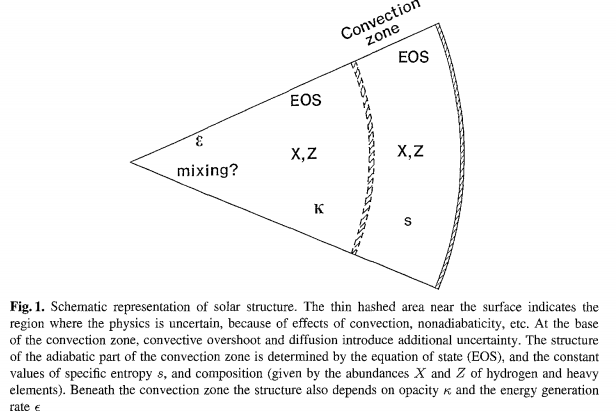
\includegraphics[width=(\textwidth),height=(\textheight-11mm),keepaspectratio]{SchemSstructure}
\caption{struttura schematica sole}
\end{figure}
\end{comment}

La luminosit\'a dipende fortemente dal valore di $Y_0$,  mentre il raggio da $\alpha$, parametro che regola l'efficienza del trasporto convettivo nella regione esterna caratterizzata fisicamente dall'entropia il cui valore \'e determinato, a meno di una costante additiva, dalla zona superadiabatica vicino alla superficie. Infatti, in un modello semplificato in cui si descrive la zona convettiva con stratificazione quasi-adiabatica tramite $P=K\rho\expy{\gamma}$, l'eccesso di entropia specifica tra la fotosfera e la parte quasi-adiabatica
\begin{equation}
\Delta S=\int_{\ln{P_{Ph}}}^{\ln{P^*}} c_P(\nabla-\nabla_a)\,d\ln{P}
\end{equation}
con $P^*$ tale che $\nabla-\nad{}\ll1$, parametrizza la variazione di $\rsun{}$ e della profondit\'a della zona convettiva, essendo $\delta\ln{K}\approx\frac{5}{3}\frac{\delta(\Delta s)}{c_P}$:
\begin{align}
&\frac{\delta R}{R}\approx 0.24\,\delta\ln{K}\approx-0.24\,\delta\ln{\alpha}\\
&\frac{\delta d_{cz}}{R}\approx-0.02\,\delta\ln{K}&\intertext{cio\'e la calibrazione del raggio influenza poco la profondit\'a della zona convettiva.}\nonumber
\end{align}
%\cite{chr97effects}
Scelgo $Y_0$ e $\alpha$ che forniscono luminosit\'a e raggio $\rsun{}=\SI{6.96e8}{\meter}$ attuali del Sole: risulta $\frac{R_b}{\rsun{}}\approx0.710$ e il valore di $Y_0=0.250$.

\clearpage

\subsection{Mean free path of plasma particles}

\cite{pit12kinetics}

\begin{definition}{Almost ideal plasma}
Suffiently rarefied to apply equation of transport to it.
\begin{equation*}
kT\gg \frac{e^2}{\overline{r}}\approx e^2n\expy{\frac{1}{3}}
\end{equation*}
\end{definition}

\begin{definition}{Debye length}
\begin{equation*}
\frac{1}{a^2}=(\frac{4\pi}{T})\sum_an_a(z_ae)^2
\end{equation*}
\end{definition}

Pg .184

\begin{usefull}{Ion-ion mean free path}
Ion-Ion collision mean free path
\begin{align*}
&l_i\approx \frac{T_i^2}{4\pi e^4 n L_i}\\
&L_i=\log{\frac{aT_i}{e^2}}&\intu{Coulomb logarithm\index{Coulomb logarithm}}\\
\end{align*}
\end{usefull}


\begin{usefull}{Transport coefficients}
Using kinetic theory of gas
\begin{itemize}
\item Electrical conductivity $\sigma$. 
\begin{align*}
&v\approx\tau e\frac{E}{m},\ j\approx env\\
&\sigma\approx\frac{e^2n\tau}{m}\approx\frac{e^2nl}{mv_T}\\
&\sigma\approx \frac{T_e\expy{\frac{3}{2}}}{e^2m\expy{\frac{1}{2}}L_e}\\
\end{align*}

\item Therma conductivity: electron play the main part.
\begin{align*}
&\kappa\approx n_el_ev_{T_e}c_e\, c_e\approx1
&\kappa\approx\frac{T_e\expy{\frac{5}{2}}}{e^4m\expy{\frac{1}{2}}L_e}
\end{align*}

\item the viscosity is mainly due to ions since they carry most of the momentum; moreover is almost unchanged after collision with electron. we consider ii only:
\begin{align*}
&\eta\approx n_iMl_iv_{T_i}\\
&\eta\approx M\expy{\frac{1}{2}}\frac{T_e\expy{\frac{5}{2}}}{e^4L_i}
\end{align*}
\end{itemize}

\end{usefull}

\subsection{Processi di diffusione.}

Nei modelli solari standard i processi di diffusione non sono generalmente inclusi ma modelli con diffusione forniscono risultati pi\'u aderenti alle frequenze osservate.


I processi di diffusione inglobano diversi effetti: la gravit\'a tende a concentrare gli elementi pi\'u pesanti verso il centro, il campo elettrico mantiene gli elettroni ancorati ai nuclei, la diffusione termica concentra le particelle pi\'u cariche e pi\'u pesanti nelle zone pi\'u calde, mentre la diffusione proporzionale al gradiente di concentrazione $C_s=\frac{n_s}{n_e}$ diminuisce le disomogeneit\'a.

Definisco il parametro di plasma per specie s,t:
\begin{align}
&\Lambda_{st}=\frac{3KTr_D}{|e_se_t|}\\
&r_D=\sqrt{\frac{KT}{4\pi\sum_sn_se_s^2}}
\end{align}
che indica il grado di interazione tra le due specie.


\begin{todo}{Inhomogeneities nuil up base convection zone.}
In models that incorporate the diffusion and
gravitational settling of helium and heavy-elements, the abundances of these
elements build up below the convection-zone base.
\end{todo}

Processi di diffusione modificano l'abbondanza degli elementi, il peso molecolare medio e l'opacit\'a. Sebbene il tempo caratteristico per percorre un raggio solare si relativamente lungo $\tau_{diff}\approx\SI{6e13}{\year}$ i processi di diffusione sono apprezzabili rispetto SSM con/senza, in particolare:

\begin{itemize}
    \item Diminuzione della profondit\'a della zona convettiva circa $2\%$.
    \item Abbondanza He iniziale $+0.4\%$ nei modelli con diffusione.
    \item La diminuzione di He rispetto ad H comporta un'aumento delle stime di Z rispetto ad H del $3\%$.
\end{itemize}

Le differenze nella struttura interna hanno effetto sulle frequenze di oscillazione predette per circa \SIrange{1}{5}{\micro\hertz}.

\begin{comment}
\begin{figure}[!ht]
\centering
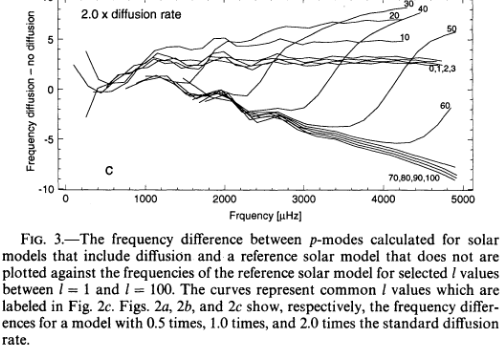
\includegraphics[width=(\textwidth),height=(\textheight-11mm),keepaspectratio]{diffusionDnu}
\caption{Differneza nelle frequenze previste.}
\end{figure}
\end{comment}

Differenze nelle frequenze calcolate per modelli con/senza diffusione:
\begin{itemize}
    \item Effetto della diffusione sui modi p \'e proporzionale al coefficiente di diffusione.
    \item Aumente frequenze modi p di basso grado nell'intero range \SIrange{1000}{4500}{\micro\hertz}.
    \item Diminuisce di \SIrange{1}{5}{\micro\hertz} le frequenze dei modi p di alto grado.
    \item Le differenze nei modi p di grado intermedio son determinate dal grado di penetrazione oltre il fondo della zona convettiva.
\end{itemize}

\clearpage

\subsection{Helioseismically constrained model}

\subsubsection{Helioseismology, solar models and NF (innocenti97)}

Il valore dell atemperatura centrale \'e determinato da opacit\'a $\kappa$ e $\frac{Z}{X}$: we allow that both are rescaled by multiplicative factor with respect to value used in SSM, these scaling factors then determined by helioseismic constraints on convective envelope.

\subsubsection{Solar model from helioseismology (Dziembowski90)}

Having determined $P(r)$ and $\rho(r)$ in the Sun's interior we can attemnpt to construct a comlpete helioseismologica model assuming

\begin{itemize}
    \item thermal equilibrium
    \item $T(\rho,P,X)$
    \item opacity in the form $\kappa(\rho,T,X)$
    \item Nuclear energy generation rate $\epsilon(\rho,T,X)$.
    
    But in outer part of solar core $He\indices{^3}$ content cannot be determinedfrom equilibrium condition.
\end{itemize}

\chapter{Equazione di stato}
\PartialToc

Le correzioni alle grandezze termodinamiche si esprimono tramite $x=\frac{l_L}{r_D}$ con

\begin{equation*}
r_D=\sqrt{\frac{KT}{4\pi\sum_sn_se_s^2}},\ l_L=\frac{e^2}{KT}
\end{equation*}

e in particolare la correzione alla pressione risulta negativa:

\begin{align*}
&P_{ES}=\frac{1}{3}U_{ES}<0\shortintertext{con}\nonumber\\
&U_{ES}=\sum eZ\overline{n}_ZV_{ES}=-\frac{e^3(\sum Z^2\overline{n}_Z)\expy{\frac{3}{2}}}{2(4\pi\epsilon_0)(\epsilon_0KT)\expy{\frac{1}{2}}}
\end{align*}

Il contributo degli elettroni, detta $n_e$ la densit\'a numerica, $\psi=\frac{KT}{KT_F}\approx\num{3e-6}T(\frac{\mu_e}{\rho})\expy{\frac{2}{3}}$ il parametro di degenerazione e $u_k$ energia cinetica dell'elettrone, \'e determinato da
\begin{align}
&\rho N_A\frac{1+X}{2}=\intzi{}\frac{8\pi p^2\,dp}{h^3(\exp{\frac{u_k}{KT}-\psi}+1)},\ \beta P-\rho\gasconstant{}(X+\frac{Y}{4}+\frac{Z}{\exv{A_Z}})=\frac{1}{3}\intzi{}pn_e\TDy{p}{u_k}\,dp\shortintertext{dove ho introdotto il peso atomico medio per elettrone libero (ionizzato) $\mu_e$ con}\nonumber
&\frac{1}{\mu_e}\approx X+\frac{1}{2}Y+\frac{1}{2}(1-X-Y)=\frac{1+X}{2}
\end{align}

\stopcontents[chapters]

\end{document}